% TODO: We need to explain JARS

\section{Static data}
\label{sec:static-data}

% TODO: mira a ver si se te ocurre un ejemplo mejor que una constante
%   o un contador de objectos. 
%       Con los métodos es más fácil: pure functions

% Math
% System

\section{The main method}
\label{sec:main-method}

As we leave Groovy behind and move into full-flavour Java, we need a
way to launch our program: a starting point. It is all too well to
have a lot of Java classes, each of them in their own \verb+.java+
file, but this is of little use if we cannot start our program from
the command like (or clicking on an icon, for that matter). 

In Groovy, we did not need an entry point. The programs or scripts
were their own entry point. We only needed to 
write \verb+groovy myScript.groovy+ and Groovy would
start the execution. The situation is slightly more complex in Java
because all files are classes, not scripts. We need to have an entry
point, a place in the code where Java knows the execution of the
program can start. This entry point is the \verb+main+ method. The
main method is a normal method of a class, and every class can have
one. It looks like this: 

\begin{verbatim}
    public static void main(String[] args) {
      // Here be the code to launch the program
    }
\end{verbatim}

If a class has a main method, it can be run from the operating system
by typing: 

\begin{verbatim}
    > java myClass
\end{verbatim}

assuming that there is a \verb+myClass.class+ file. The 
signature of the \verb+main+ method is a bit long, but we have
already learnt what each of its elements means: 

\begin{itemize}
\item It must be \verb+public+, because otherwise it cannot be
  accessed from outside the class (and how would the program launch
  then?).
\item It must be \verb+static+, because it pertains to the class, not
  to each of its objects.
\item It returns \verb+void+. This is a method that is never called by
  other classes, so a return type is unnecessary.
\item The only parameter is a 1-D array of Strings, called \verb+args+
  (short for arguments). Actually the name is not important. The
  elements in the array are the parameters passed in the command line,
  if any. For example, if you run a program with a line like
  \verb+java myClass www.google.com 80 true+, the first element
  (i.e.~args[0]) of \verb+args+ will be ``www.google.com'', the second
  element will be ``80'', and the third one will be ``true''. If you
  want to use these parameters with a different type you need to parse
  them. 
\end{itemize}

\subsection{Liberating your main method from static restrictions}
\label{sec:liber-your-launch}

As static code does not understand anything about instance
(i.e.~non-static) methods or data, you will not be able to use your
instance data from your main method. This seems restricting at first,
as in the following example: imagine that we want to start a program
from a BitTorrentDownloader class, and we want to give the name of the
host and the port from the command line

\begin{verbatim}
    public class BitTorrentDownloader {
        private String host;
        private int port;
    
        public BitTorrentDownloader(String host, int port) {
            this.host = host;
            this.port = port;
        }
    
        public static void main(String[] args) {
            host = args[0];
            port = Integer.parseInt(args[1]);
            // with the fields initialised, 
            // launching code comes here...
            // ...
        }
    }
\end{verbatim}

When you try to compile this program, java will complain with the
following error: 

\begin{verbatim}
    non-static variables cannot be referenced from a static context
    host = args[0];
    ^
    port = Integer.parseInt(args[1]);
    ^
\end{verbatim}

One (bad) solution is to make \verb+host+ and \verb+port+ static, but
that means that there can only be one of each. This is usually a bad
idea in the long run. Maybe in a future version you will like several
BitTorrentDownloaders working in parallel, or maybe you would to
launch many at the same time and put them in a queue. All of this
would be impossible if the fields were static. Remember: \verb+static+
means ``only one per class'', and programmer usually like to have as
many as possible of everything, just in case. As a rule of thumb,
\textbf{never make anything ``static'' unless it is absolutely necessary}.

There is another (much better) solution: to instantiate the class
inside it main method, and then run all the code from a non-static
launching method. This method is commonly called \verb+run()+ or
\verb+launch()+. See the example: 

\begin{verbatim}
    public class BitTorrentDownloader {
        private String host;
        private int port;
    
        public BitTorrentDownloader(String host, int port) {
            this.host = host;
            this.port = port;
        }
    
        public static void main(String[] args) {
            String host = args[0];
            int port = Integer.parseInt(args[1]);
            BitTorrentDownloader downloader = new BitTorrentDownloader(host, port);
            downloader.launch();
        }

        private void launch() {
            // with the fields initialised, 
            // launching code comes here...
            // ...
        }
    }
\end{verbatim}

\section{More differences between Groovy and Java}
\label{sec:more-diff-betw}

\subsection{String.equals != ==}
\label{sec:string.equals-=-==}

In Groovy we have become used to comparing String using ``==''. In
Java we have to be careful and use the method
\verb+.equals()+. Otherwise we may get funny results like in the
following simple code: 

\begin{verbatim}
    System.out.print("Enter a string: ");
    String str1 = System.console().readLine();
    System.out.print("Enter another string: ");
    String str2 = System.console().readLine();
    System.out.println("Are '" + str1 + "' and '" + str2 + "' the same?");
    System.out.println("Using ==: " + (str1 == str2));
    System.out.println("Using .equals(): " + (str1.equals(str2)));
\end{verbatim}

that produces the following output: 

\begin{verbatim}
    Enter a string: This is a String
    Enter another string: This is a String
    Are 'This is a String' and 'This is a String' the same?
    Using ==: false
    Using .equals(): true
\end{verbatim}

This is because the equality operator ``=='' only works with simple
types, with little ``boxes''. When it is used to compare objects like
Strings, it compares the pointers not the contents of the objects (see
Figure~\ref{fig:equals}). The
method \verb+.equals()+, on the other hand, can be used to compare the
content of the objects. 

\begin{figure}[bthp]
  \centering
  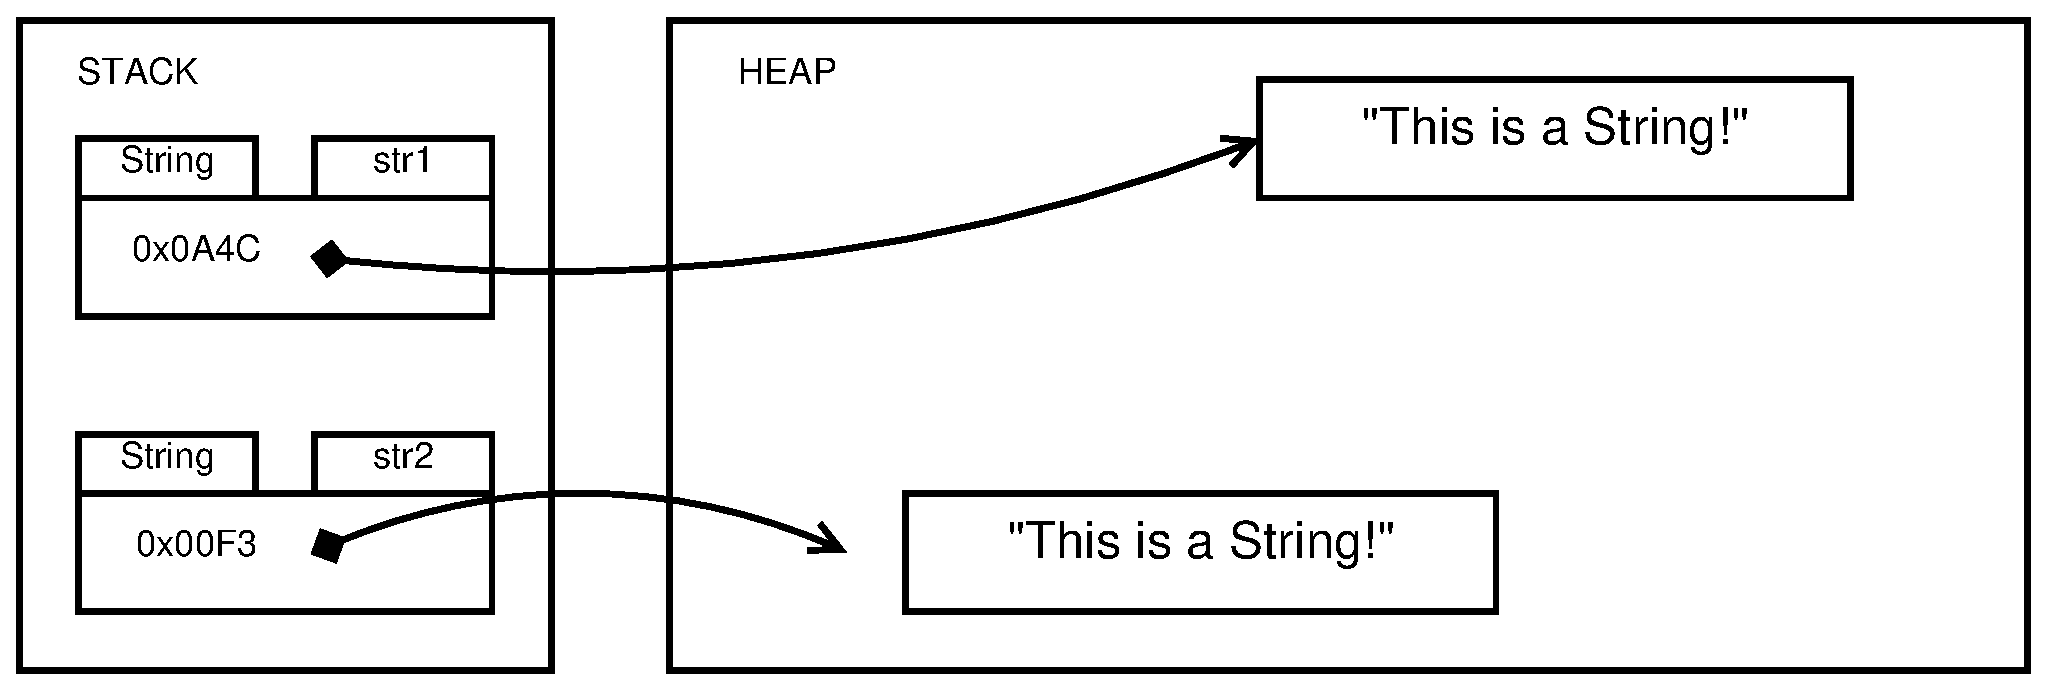
\includegraphics[width=\textwidth]{gfx/variables-string-equals}
  \caption{The operator ``=='' compares simple types. When used to
    compare complex types, it compares just the pointers.} 
  \label{fig:equals}
\end{figure}

As a rule of thumb, \textbf{always use the method .equals()
  when comparing Strings} or any other complex types in Java.

\paragraph{Note.}
\label{sec:notre}

For some classes, the effect of \verb+.equals()+ is the same as
``=='', i.e.~it compares the pointers and not the content of the
objects. This depends on the class and its semantics. For instance,
we usually think that two Strings or two Integers (class, not simple
type) are the same if they have the same content, but we do not think
of two \verb+Person+ to be same even if they have the same name. We
will learn more about this when we learn about class inheritance but,
for now, it suffices to say that objects should always be compared
with \verb+equals()+ and not with ``==''. The operator ``=='' should
only be used for simple types (also known as \emph{primitive} types). 

\subsection{A new type of loop: do\ldots while}
\label{sec:new-type-loop}

With a loop you can perform the same operations over and over
again. However, if the condition for the loop is never true a
\texttt{while} loop will never run; and sometimes you need it to run
at least once, like in this case:

\begin{verbatim}
    System.out.println("Enter the names of your friends. Finish by typing END.");
    String name = System.console().readLine();
    System.out.println(s + ": friend");
    while (!s.equals("END")) {
        System.out.println(s + ": friend";
        name = System.console().readLine();
    }
\end{verbatim}

In this brief example you need to repeat the same code to read input
from the user in two different places. If
the only way to do loops was using \texttt{while}, this repetition
could not be avoided (and in a less trivial program, with
intelligent error-checking and the like, this could be a lot of
repetition!). Fortunately, in Java we can use 
the \texttt{do\ldots while} loop: 

\begin{verbatim}
    System.out.println("Enter the names of your friends. Finish by typing END.");
    do {
        String name = System.console().readLine();
        System.out.println(name + ": friend");
    } while (!name.equals("END"));
\end{verbatim}


Remember, repeated code is usually a bad sign: a symptom of poor
design and/or poor programming. When you have the same code in two
different places, and make a change in one of them, it is very easy to
forget to change the other too\ldots a common source of bugs for
careless programmers. If you notice you have repeated code in your
program, think twice about a better way of doing things, without
repetition. Remember the DRY principle: \textbf{Don't Repeat
  Yourself}. Keep it in mind at all times.


\subsubsection*{Exercise}

Make a class that implements a method 
that reads a list of marks between 0 and 100 from the
user, one per line, and stops when the user introduces a -1. The
program should output at the end (and only at the end) how many marks
there were in total, how many were distinctions (70--100), how many
were passes (50--69), how many failed (0--49), and how many were
invalid (e.g. 150 or -3). Use \texttt{readLine()} exactly once.



%%% Local Variables:
%%% mode: latex
%%% TeX-master: "main"
%%% End:
